\newpage
\appendix
\chapter{Apêndice 1}
\label{apendice1}

\section{Técnicas e Métodos da Engenharia de Usabilidade}

Esta seção mostra as técnicas e os métodos que são utilizados pela interação humano computador para desenvolver um sistema com usabilidade.
%
De acordo com \\ ~\citeonline{bervian2002metodologia} as técnicas são procedimentos específicos utilizados por uma ciência determinada. O conjunto com várias técnicas constituem os métodos. Algumas técnicas são utilizadas em várias ciências e os métodos se adapta às diversas ciências a medida que há imposição de uso de técnicas especializadas.
%
~\citeonline{cybis2010} divide as técnicas e os métodos da engenharia de usabilidade em três tipos: Concepção, Análise e Avaliação.


\subsection{Métodos e técnicas de concepção}

	Os métodos de concepção são utilizados para implementar as especificações e os requisitos para a interface a usabilidade de um sistema.

\begin{description}

\item[Brainstorming:]

	Bastante utilizado em ambientes ágeis para obter ideias, entrar em consenso sobre problemas ou novas propostas.

\item[Storyboard:]

É uma representação das interações entre os usuários e o sistema em seu ambiente de trabalho. Corresponde ao detalhamento de um cenário de uso especificado para o sistema consistindo em uma sequência de desenhos representando não só os esboços de telas, mas também os elementos do contexto (usuários, equipamentos, móveis, telefones, colegas).

\item[Card Sorting:]

	É uma técnica usada para descobrir como o usuário classifica determinada informação em sua mente. O usuário recebe uma série de cartões embaralhados descrevendo conteúdos e agrupam os cartões que tenham alguma relação. Podem ser distribuídos cartões com nomes de categorias. 
%
O \textit{card sorting} pode ser aberto ou fechado podendo ser aplicado tanto de forma presencial ou remota e aplicados para grupos ou para uma única pessoa. Recomenda-se no mínimo 15 testes e que cada teste tenha 2 pessoas.\footnote{\url{www.uxdesign.blog.br}}
	
\item[Diagramas de Afinidade:]

	São utilizados para organizar uma grande quantidade de itens em grupos lógicos. Diferente do \textit{card sorting}, nesta técnica os projetistas e usuários trabalham juntos para obter consenso sobre a organização dos itens. Essa técnica pode ser usada para analisar os resultados de estudos de campo e analisar as conclusões de uma avaliação de usabilidade.

\item[Protótipos:]

	Os protótipos de papel são úteis para detectar problemas de usabilidade logo no início do proceso de \emph{design}. São usados para esclarecer os requisitos específicos para o projeto da interface do sistema. São rápidos de construir, permitindo rápidas interações de projeto e necessitam de poucos recursos para serem criados. 
	Existem também os protótipos de baixa, média e alta que simulam o sistema com mais fidelidade do que os protótipos em papel. 
\end{description}

%------------------------------------------------------------%%%

\subsection{Métodos e técnicas de análise}

Estes métodos são utilizados para buscar informações sobre o contexto de uso e sobre a usabilidade de um sistema. Podem ser feitas análises do perfil do usuário, o ambiente de uso, as tarefas, possibilidades e restrições do sistema.

As técnicas mencionadas à baixo visam apoiar os projetistas de interface na busca de informações sobre o contexto de uso e sobre a usabilidade de um sistema existente. Essas técnicas são empregadas de forma que se complementem-se umas as outras.

\begin{description}

\item[Observação:]

	Essa técnica caracteriza-se por um pesquisador observando o usuário e tomando notas, enquanto este trabalha em seu contexto usual. É uma técnica útil para obter dados quantitativos (tempo para as tarefas) e qualitativos (práticas e estratégias do usuário). No planejamento é importante definir os objetivos e as maneiras de como será registrada os acontecimentos. Deve-se levar em consideração o fato que muitos usuários por estarem sendo observados podem alterar seu comportamento ao utilizar a ferramenta. É importante que todos estejam cientes dos objetivos do estudo, deixando claro que não é ele que será avaliado e sim conhecer uma situação de uso ~\cite{cybis2010}.

\item[Entrevistas Tradicionais:]

Através de entrevistas podemos obter as opiniões tanto dos usuários atuais como dos futuros usuários dos sistemas. Primeiramente é importante identificar as necessidades das pessoas em acessar uma determinada informação.

\item[Eyetracking:]

É uma técnica que rastreia o movimento dos olhos e da cabeça para registrar a tomada de informações numa interface.

\item[Questionários de Perfil de Uso:]
 
É utilizado para obter informações sobre as características reais dos usuários de um sistema e saber como eles realmente utilizam tais ferramentas. É importante que ao utilizar os questionários de perfil de uso é preciso definir um foco para a sua pesquisa. Deve-se identificar as principais dúvidas da equipe de projeto em relação ao uso do sistema ~\cite{cybis2010}.

Este tipo de questionário pode ser enviado para os \textit{e-mails} dos usuários da ferramenta em análise. É importante definir o tamanho de sua amostra. De acordo com ~\citeonline{cybis2010}, de 20 a 30 por cento é a taxa de retorno dos questionários enviados. As respostas podem ser analisadas utilizando métodos estatísticos.


\item[Questionários de Satisfação:]

	A aplicação de questionários é um dos métodos mais utilizados para avaliação da satisfação do usuário. Eles resultam da avaliação subjetiva pelo usuário, o qual é influenciado pelos tipos de questões aplicadas.
	
	Questionários de satisfação são utilizados principalmente quando existem usuários experientes que utilizam o sistema com frequência, podendo ter informações fidedigna sobre aspectos satisfatórios e insatisfatórios no sistema. Também podem ser aplicados por usuários de uma nova versão de um sistema imediatamente após um teste de usabilidade. Essa relação com os testes de usabilidade é interessante por permitir a correlação das medidas de desempenho (tempo, frequência) com as medidas de satisfação do usuário ~\cite{cybis2010}.

	É recomendado que se utilize um questionário padronizado, pois permite a comparação de resultados obtidos por diferentes sistemas. Estes questionários apresentam opções de respostas fechadas, o que permite a produção de dados quantitativos e objetivos ~\cite{cybis2010}.

	Um grande número de questionários foram desenvolvidos pela comunidade científica para a avaliação da usabilidade.  Alguns exemplos de questionários são: QUIS, SUMI,  WAMMI, SUS, ASQ, PSQ, PSSUQ e CSUQ. Os detalhes referentes a cada questionário estão detalhados no apêndice~\ref{apendice1}.

\item[Grupos de Foco:]

É uma reunião informal de usuários que manifestam suas opiniões sobre o determinado assunto, que pode ser tanto uma oportunidade de novas funcionalidades ou algum problema específico.
%
Um moderador deve preparar um roteiro  com uma lista de assuntos a serem tratados. É importante que os participantes sejam de perfis diferentes para que possa ter uma maior diversidade de informações. Costuma-se ter em média de 6 a 12 usuários em uma mesa de reuniões. Os registros das informações podem ser através de vídeos ou blocos de anotações. O objetivo não é ter a obtenção do consenso em torno das ideias, mas sim ter uma boa quantidade de opiniões sobre o assunto a ser tratados ~\cite{cybis2010}.


\item[Diários:]

	É uma técnica útil quando a experiência do usuário é ampla e depende da utilização em muitos lugares. Nessa técnica os usários carregam consigo um pequeno diário para nele anotar as informações do seu dia-a-dia na utilização do sistema ~\cite{cybis2010}.

\item[Benchmarking de Usabilidade:]

	Definido como método sistemático e contínuo de avaliação de sistemas reconhecidos como representantes das melhores e mais eficazes práticas com a finalidade de comparar desempenhos e identificar oportunidades de melhoria ~\cite{spendolini1994}.

	Esse método parte da definição dos critérios de avaliação e seleção de representantes relevantes para criar uma listagem de características desejáveis para o futuro sistema, como também os aspectos que são desfavoráveis e que devem ser evitados.

\item[Cenários de uso:]

	É uma técnica simples e eficaz para analisar e comunicar uma parte das especificações de requisitos produzidos para a usabilidade e a interface. São utilizados para comunicar os cenários atuais de uma tarefa (problema) e o cenário futuro (solução). Os cenários de solução deve descrever em linguagem natural, como determinados usuários realizarão tarefas específicas com o sistema em um determinado contexto. É preciso decompor os objetivos dos usuários segundo as operações necessárias para alcança-los, identificando as atividades que serão realizadas pelos usuários ~\cite{cybis2010}.

\item[Personas:]

	A técnica de persona descreve o perfil de uma pessoa fictícia envolvida com o produto. Trata-se de inventar um conjunto de pessoas (três ou quatro) que estejam dentro da população de usuários pretendidos e descrevê-las em detalhes.
%
	As informações devem ser qualitativas e coletadas por meio de entrevistas e questionários junto à população alvo do sistema. As personas permitem maior entendimento dos usuários, colocando-os no centro das decisões do projeto. Essa técnica tem objetivos similares aos de cenários, porém ao invés do foco ser na tarefa, deve-se ter foco em uma pessoa que faça parte do público alvo do sistema ~\cite{cybis2010}.

\end{description}

\subsection{Técnicas e Métodos de avaliação}

\begin{description}

\item[Checklists:]

	É uma técnica de inspeção que oferece uma maneira de abordagem rápida, fácil e de baixo custo para a avaliação de uma interface. Permite com que usuários que não são especialistas em ergonomia identificarem problemas menores e repetitivos ~\cite{cybis2010}.
%
Várias vantagens são encontradas na utilização dessa técnica como: redução de custos de avaliação por não precisar de especialistas; sistematização das avaliações; reduz a subjetividade dos processos de avaliação e fornece um conhecimento ergonômico sobre o que avaliar.
%
O Ergolist \footnote{\url{http://www.labiutil.inf.ufsc.br/ergolist/check.htm}} é um aplicativo que pode ser utilizado para realizar uma inspeção da qualidade ergonômica da interface com o usuário do sistema.

\item[Avaliação heurística:]

	Representa um julgamento de valor sobre as qualidades ergonômicas das interfaces Humano-Computador. Essa avaliação é realizada por especialistas em ergonomia e usabilidade. Eles examinam o sistema interativo e diagnosticam os problemas ou as barreiras que os usuários provavelmente encontrarão durante a interação ~\cite{cybis2010}.

	O principal objetivo desse tipo de avaliação é avaliar a interface em fases iniciais do sistema, sem o envolvimento do usuário. Os graves problemas de interface devem ser localizados antes que realizem os testes de usabilidade com usuários reais ~\cite{santos2012}.

	As avaliações mais utilizadas são as 10 heurísticas de ~\citeonline{nielsen1994}. São elas:

	\begin{itemize}
		\item{Visibilidade de acordo com o sistema}
		\item{Mapeamento entre o sistema e o mundo real}
		\item{Liberdade e controle ao usuário}
		\item{Consistência e Padrões}
		\item{Prevenção de Erros}
		\item{Reconhecer em vez de relembrar}
		\item{Flexibilidade e Eficiência de uso}
		\item{Design estético e minimalista}
		\item{Suporte para usuário reconhecer, diagnosticar e recuperar erros}
		\item{Ajuda e documentação}
	\end{itemize}


	Pesquisas realizadas por Jakob Nielsen fornecem indicações sobre a quantidade de avaliadores que devem ser consultados para que possam identificar grande parte dos problemas de ergonomia. Cinco avaliadores com experiência tanto em usabilidade como no sistema consegue identificar 95 por cento dos problemas de ergonomia enquanto especialistas que conhece apenas de usabilidade identificam 85 por cento.

\begin{figure}[h]
    \centering
    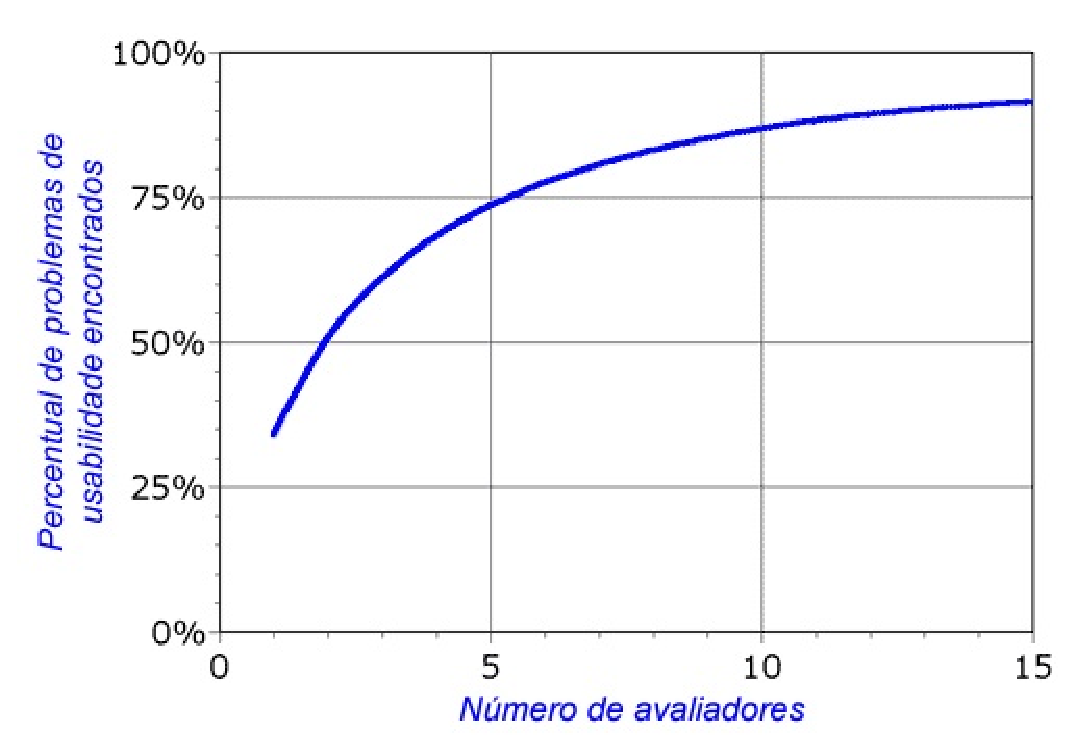
\includegraphics[keepaspectratio=true,scale=0.60]
      {figuras/avaliadores_heuristica.eps}
    \caption{Número de avaliadores~\cite{nielsen1994}}
    \label{avaliadores}
\end{figure}

	A avaliação heurística requer pouco planejamento e pode fazer parte de um processo interativo de um projeto e aplicado em todas as fases de desenvolvimento da interface, mas é preciso que seja avaliado por especialistas de usabilidade com pleno conhecimento nas heurísticas.
	

\item[Listas de Verificação:]

	Permitem que profissionais que não necessariamente sejam especialistas em ergonomia identifiquem problemas menores e repetitivos das interfaces. As normas ISO 9241, partes 10 a 17, fornecem listas de verificação de ergonomia bem definidas, assim como as fornecidas pelo site Ergolist ~\cite{cybis2010}.
	

\item[Percurso Cognitivo:]

Percurso cognitivo é um método de inspeção de usabilidade que tem como objetivo avaliar a interface considerando a facilidade da interface. A finalidade do percurso cognitivo é fazer com que o \emph{design} de interação seja fácil de aprender por meio da exploração. Os inspetores aplicam uma lista de verificação orientada à tarefa interativa, abordando os processos cognitivos que se estabelecem quando o usuário a realiza pela primeira vez~\cite{cybis2010}.


\item[Teste de Usabilidade:]

É um dos métodos de teste de experiência do usuário (UX) mais frequentemente utilizado e conhecido entre aqueles que não são projetistas da UX. Realizar testes com usuários é o núcleo do \emph{Design} Centrado no Usuário, pois é através destes que podemos saber se as reais expectativas dos usuários são atendidas ~\cite{santos2012}.
%
O teste consiste em avaliar o desempenho dos usuários na execução de tarefas cuidadosamente preparadas, tarefas estas dentro do escopo do sistema. Esse desempenho pode ser avaliado no quesito, número de erros e tempo de execução da tarefa, questionários e entrevistas também podem ser utilizados ~\cite{preece2007}. Na próxima seção será detalhado os passos comuns que devem ser seguidos para a execução dos testes de usabilidade.


\end{description}

	As técnicas descritas nesse capítulo podem ser associadas com várias outras técnicas e para a escolha de cada técnica é importante examinar as possibilidades dos recursos necessários e os disponíveis e as expectativas de resultados da avaliação da usabilidade. Cada técnica apresentam qualidades diferentes em relação à quantidade de problemas que as identificam, sistematização dos resultados, à facilidade da aplicação. 
%
No estudo de caso detalhado e planejado no próximo capítulo, separamos algumas técnicas que podem ser utilizadas na avaliação da usabilidade e na identificação dos usuários. 



\section{Questionário de Perfil do Usuário}

	Este questionário foi utilizado para identificar o perfil do usuário e algumas de suas necessidades. 




\begin{figure}[h]
    \centering
    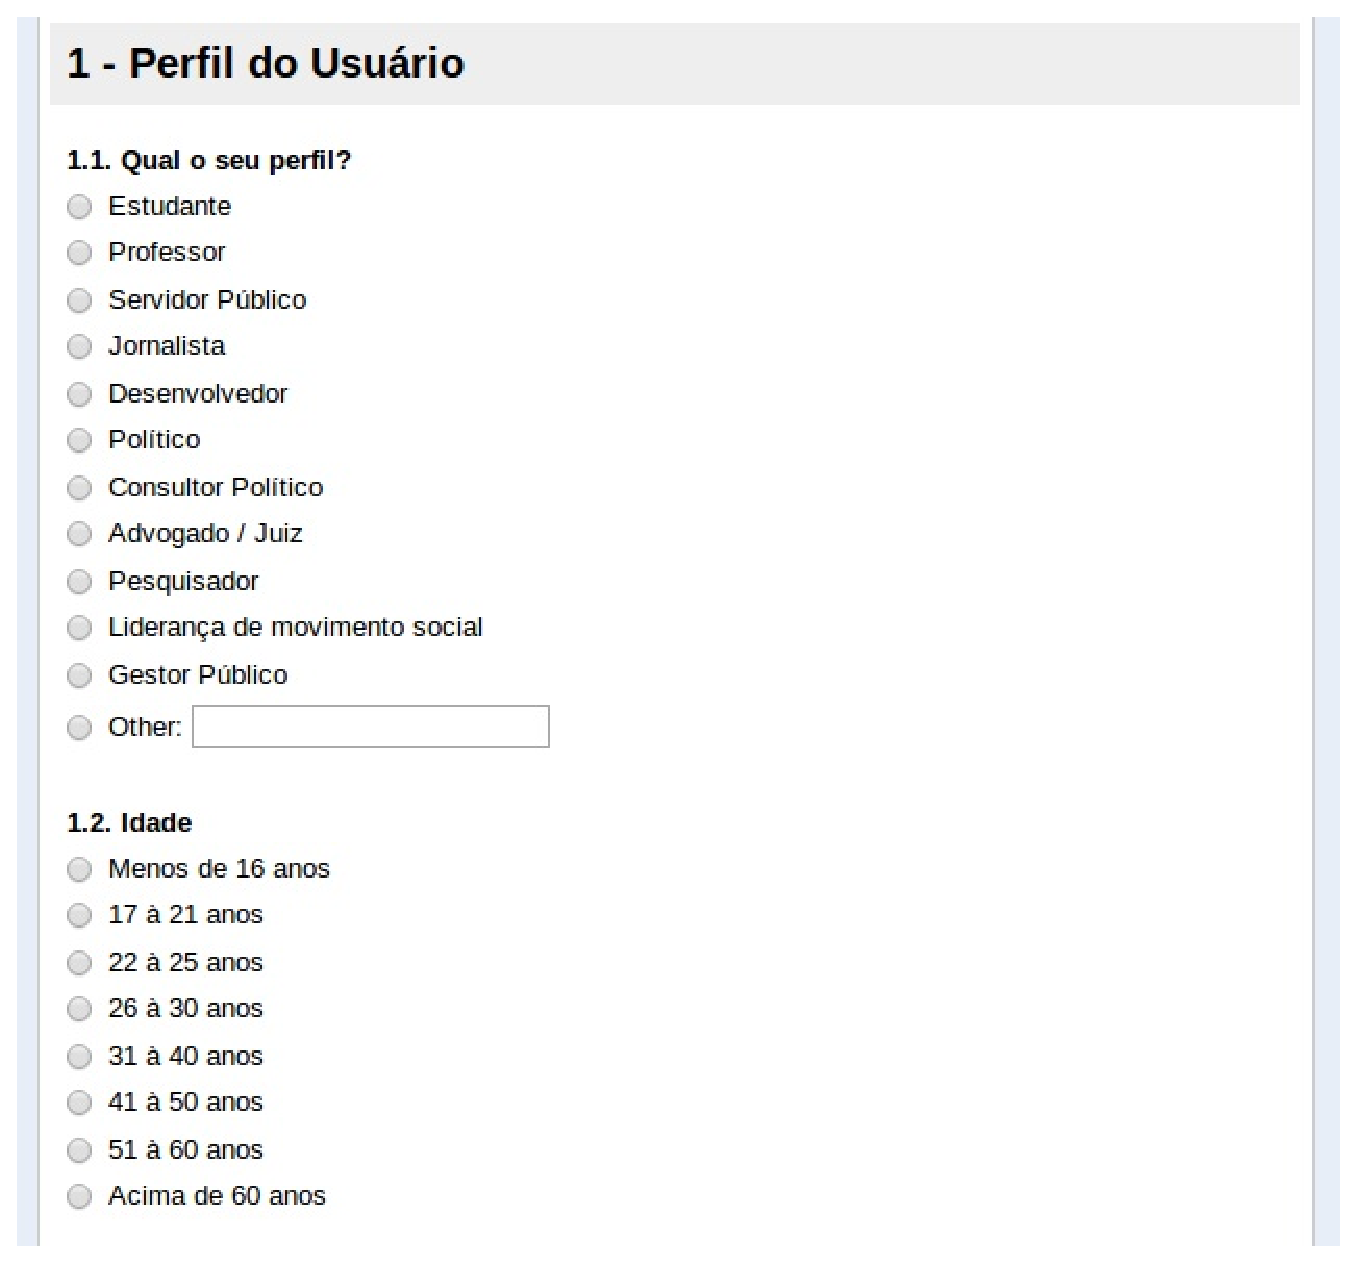
\includegraphics[keepaspectratio=true,scale=0.60]
      {figuras/perf1.eps}
	\caption{Questionário de perfil do usuário}
    \label{perfilgeral}
\end{figure}
%
%
\newpage


A primeira parte do questionário mostra perguntas gerais referentes ao perfil social dos usuários como idade, ocupação/profissão, gênero, formação  e áreas de interesse.



\begin{figure}[!h]
    \centering
    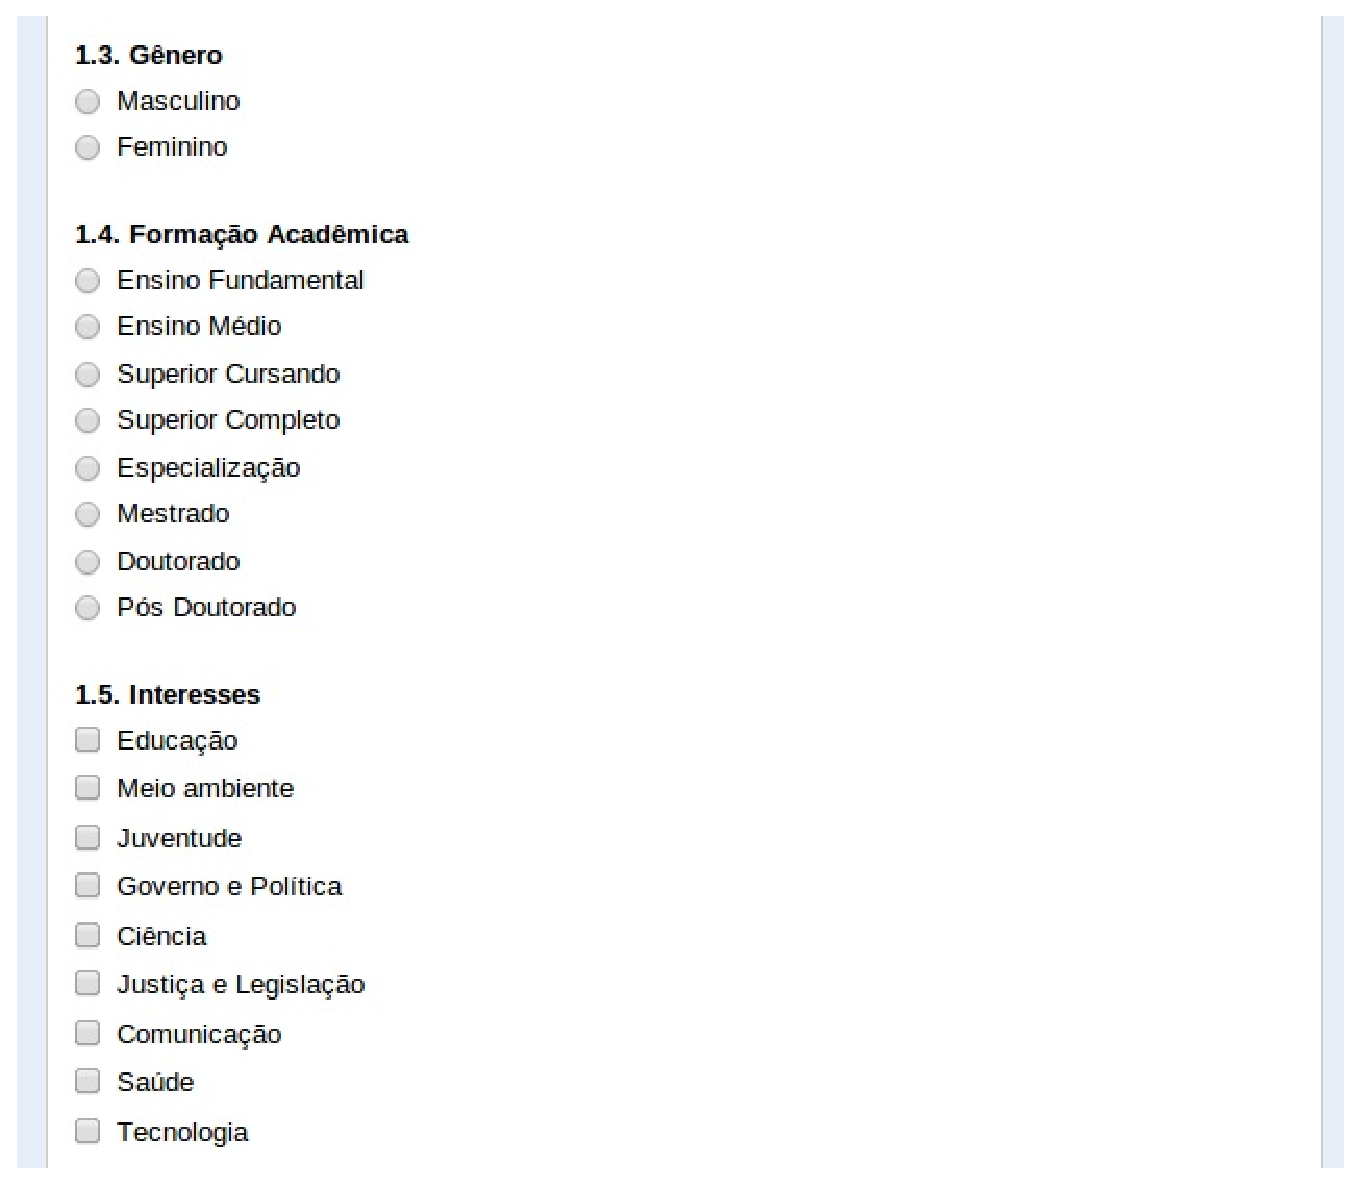
\includegraphics[keepaspectratio=true,scale=0.60]
      {figuras/perf2.eps}
     \caption{Questionário de perfil do usuário - Continuação}
    \label{perfilgeral}
\end{figure}
	
\newpage

	Na seção dois do questionário, as informações sobre o uso dos meios de comunicação que cada usuário. Informações sobre locais de acesso à internet, velocidade de conexão, principais redes sociais e as principais atividades que realiza na internet. 


\begin{figure}[!h]
    \centering
    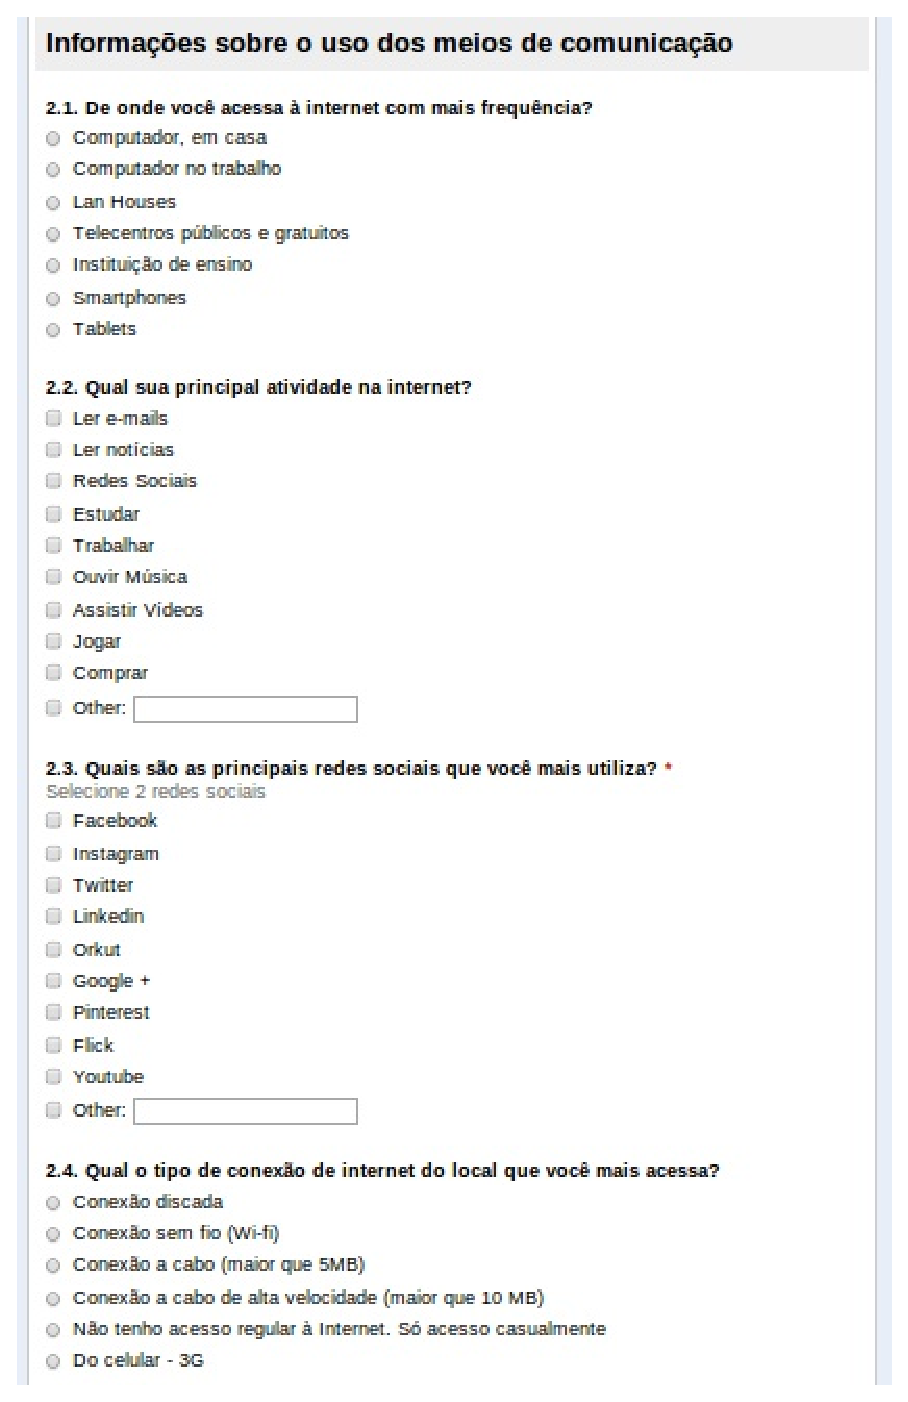
\includegraphics[keepaspectratio=true,scale=0.60]
      {figuras/perf03.eps}
    \label{meiosdecomunicaçaõ}
	\caption{Informações sobre o uso dos meios de comunicação}
\end{figure}

\newpage


	Na terceira seção do questionário são feitas perguntas referentes ao engajamento político/social dos usuários como atuações em movimentos políticos e sociais e participações em manifestações, além de saber sobre o meio de informação na qual se informa sobre os movimentos.





\begin{figure}[!h]
    \centering
    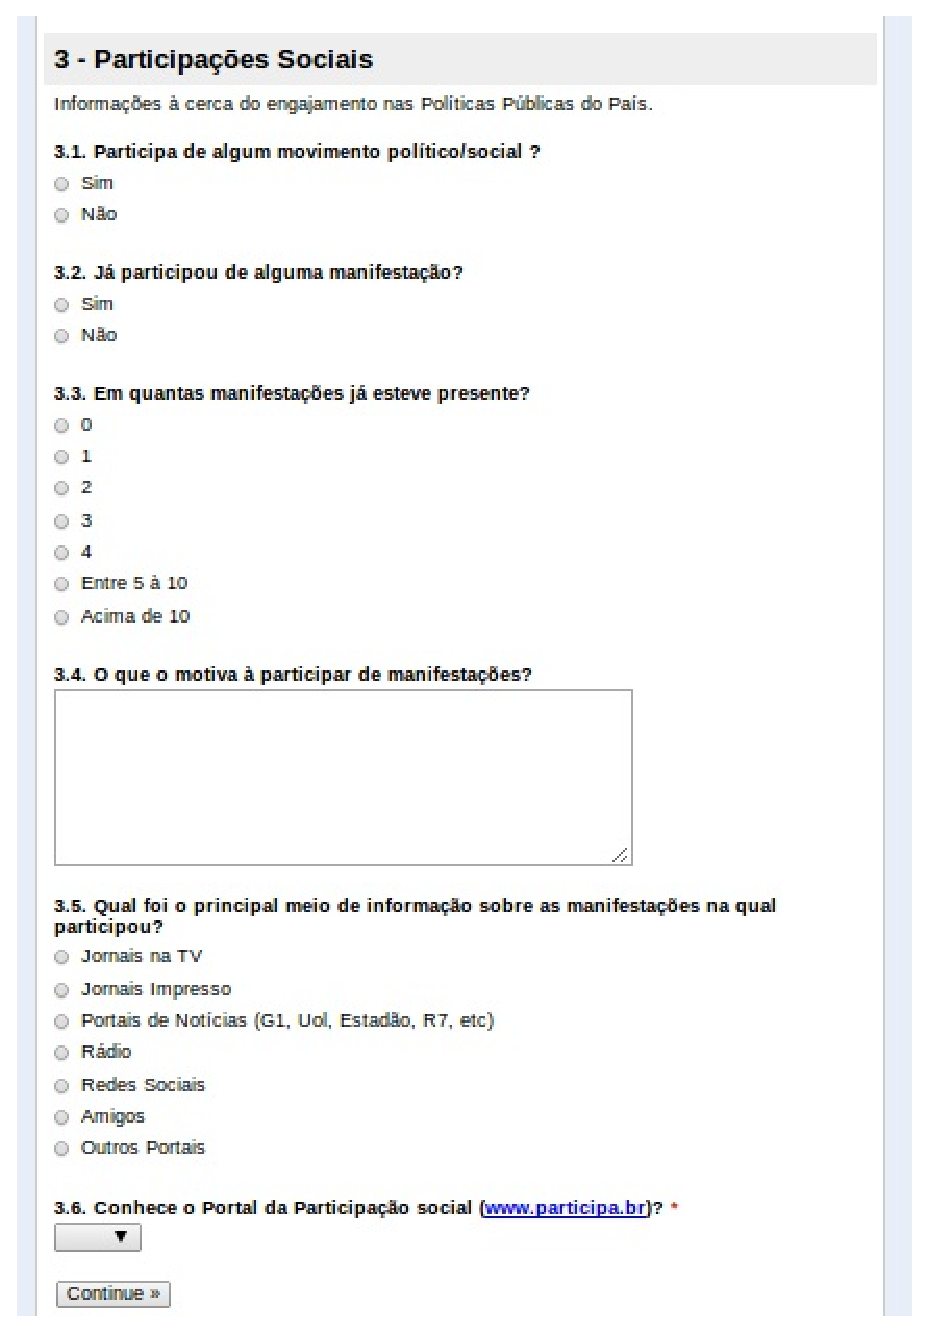
\includegraphics[keepaspectratio=true,scale=0.60]
      {figuras/perf4.eps}
    \caption{Participações sociais}
    \label{participações}
\end{figure}

\newpage

	Depois que foram preenchidas a primeira parte do questionário, os usuários que já usavam o portal da participação social iriam preencher algumas outras questões referente a utilização do portal, tentando entender as principais atividades e funcionalidades que cada usuário utilizava.




\begin{figure}[!h]
    \centering
    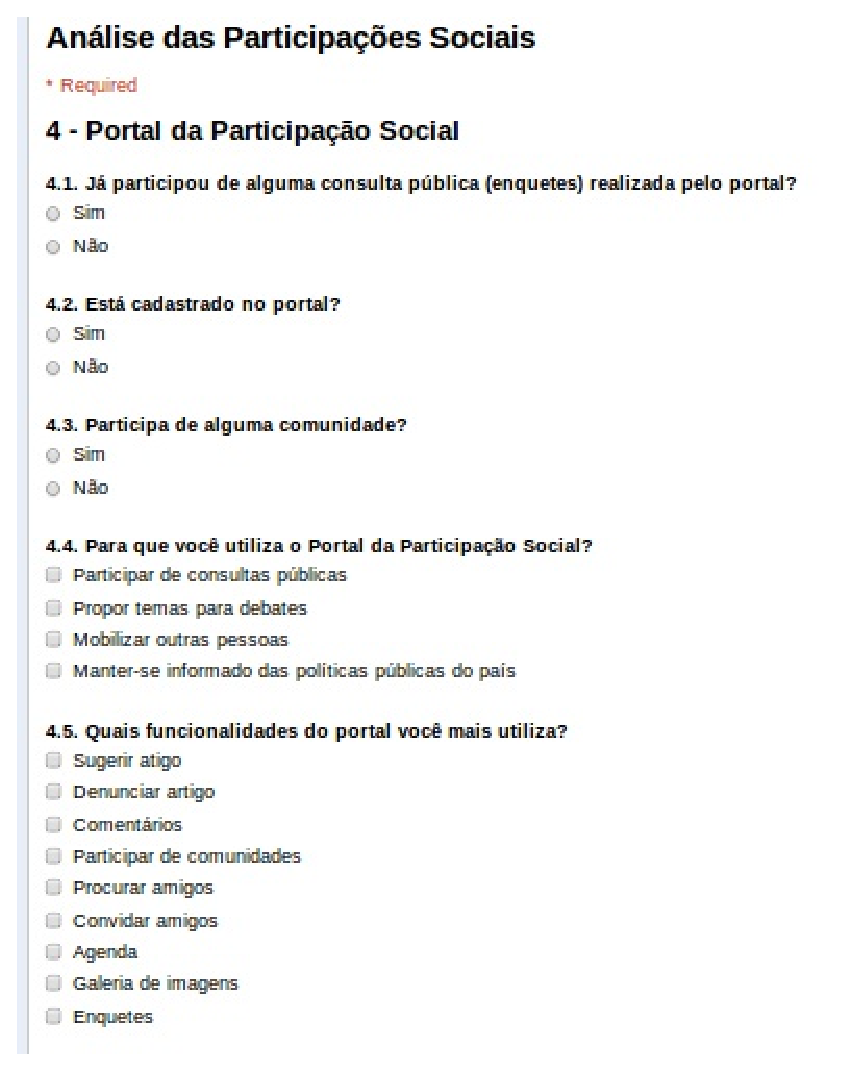
\includegraphics[keepaspectratio=true,scale=0.60]
      {figuras/perf5.eps}
    \caption{Portal da Participação Social}
    \label{participabr}
\end{figure}


\newpage

	Na seção cinco do questionário, as questões servem para conhecer o tempo e o local de acesso dos usuários do portal da participação social




\begin{figure}[!h]
    \centering
    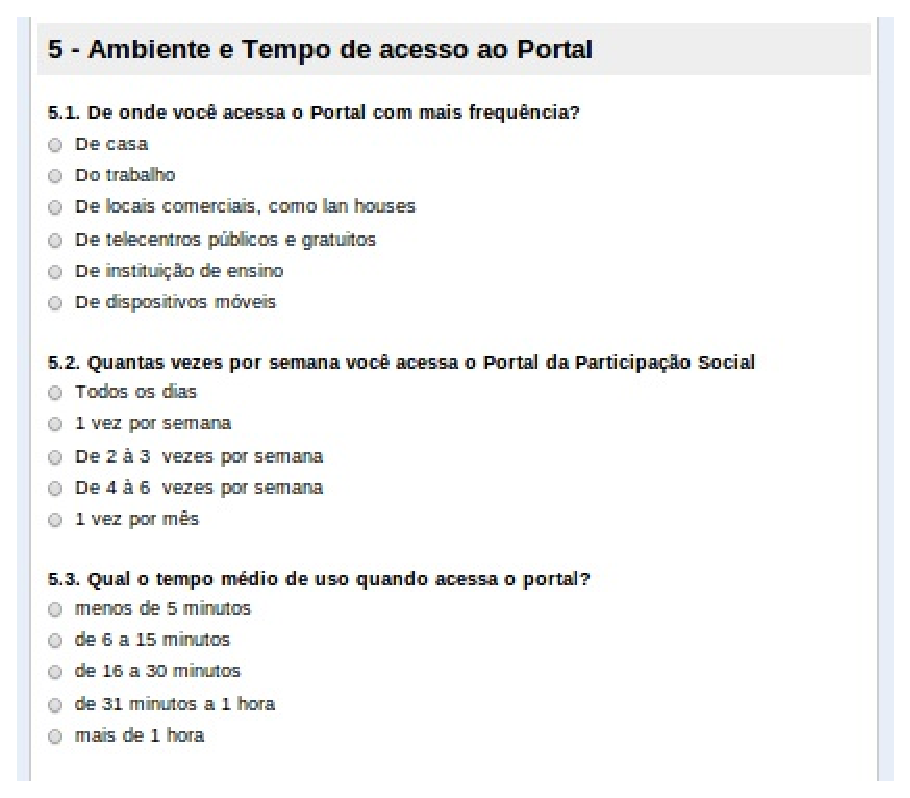
\includegraphics[keepaspectratio=true,scale=0.60]
      {figuras/perf6.eps}
    \caption{Ambiente e tempo de acesso no portal}
    \label{acessoportal}
\end{figure}

\section{Questionário de Satisfação}

	Levantamos informações sobre alguns questionários de satisfação de uso existentes na literatura e foi feito uma comparação entre cada um deles.

\subsection{QUIS - Questionnaire for User Interaction Satisfaction}

	O QUIS mede a satisfação do usuário quanto â usabilidade do produto de maneira padronizada, segura e válida, a fim de obter informações precisas em relação à reação dos usuários a novos produtos (QUIS, 2009);

	A versão atual é a QUIS 7.0 (Norman e Shneiderman, 2010), contém um questionário onde possui a avaliação da satisfação geral e avaliações de fatores específicos de interfaces organizadas hierarquicamente: tela, terminologia e retroalimentação do sistema, aprendizado, capacidades do sistema, manuais técnicos, tutoriais online, multimídia, teleconferência e instalação de software. Pode ser configurado de acordo com a necessidade e interesse do usuário. 

	É um questionário proprietário, é sugerido o uso de planilhas eletrônicas e softwares estatísticos até que se implementem recursos de análise no servidor web dos proprietários.

\subsection{SUS – System Usability Scale}

	O SUS é uma escala de usabilidade do tipo Likert que possui uma visão global e subjetiva em suas avaliações de usabilidade. Ele apresenta ao entrevistado uma lista de perguntas que devem ser respondidas em uma escala de satisfação (indica o grau de concordância ou discordância do usuário) \cite{brooke1996sus}.

	O autor se baseou na afirmação de que no contexto industrial, as avaliações completas não são práticas e requerem muito esforço e custo. O SUS foi criado pela necessidade de se ter uma avaliação de usabilidade simples e rápida. Os métodos de avaliação foram simplificados e o número de questões reduzidas, pois uma quantidade grande de questões desanima os usuários que possivelmente não preencheria todas as questões, resultando assim problemas na captura de reações subjetivas do usuário. Foi então proposto um questionário com 10 questões que utiliza a escala Likert de cinco ou sete pontos. Este questionário abrange vários aspectos da usabilidade, tais como: necessidade de suporte, treinamento e complexidade. ~\cite{preece2007}

\subsection{SUMI – Usability Measurement Inventory}

	O SUMI proposto por ~\citeonline{kirakowski1988measuring} é um questionário para medição da qualidade de um software do ponto de vista do usuário, é um método consistente usado para avaliar a qualidade de uso de um produto de software ou protótipo, e pode ajudar na descoberta de falhas de usabilidade. É mencionado na norma ISO 9241 como um método reconhecido para testar a satisfação do usuário. O SUMI é um questionário comercial. 

	Inicialmente continha 150 itens onde o participante escolhia se (concordo fortemente, concordo, não sei, discordo ou discordo totalmente). Atualmente são 50 itens divididos em 5 grupos de 10 itens. Os grupos de itens são: eficiência, afeto, eficácia, controle e aprendizado. Os entrevistados preenchem o questionário no seu local de trabalho e devem decidir entre as opções: concordo, não sei ou discordo totalmente.

\subsection{ASQ – The After-Scenario Questionnaire}

O ASQ é um questionário de três itens que são utilizados para avaliar a satisfação do usuário após a conclusão de cada cenário/tarefa. São realizadas umas séries de tarefas que estão de acordo com a realidade do usuário.Este questionário aborda questões como: facilidade de conclusão da tarefa, tempo para completar uma tarefa e adequação das informações de suporte.São questões do tipo Likert, aplicando uma escala de 1 a 7, onde 1 representa “ Concordo totalmente ” e 7 para “ Discordo totalmente ”. ~\cite{lewis1995ibm}

O participante gasta em média 1 hora pra realizar cada cenário, no fim de cada cenário é preenchido o questionário ASQ. Após completar todos os cenários, no fim de 1 dia de trabalho (8 horas), os participantes preenchem o questionário PSSUQ para avaliação geral do sistema.O ASQ foi aplicado na IBM por diferentes tipos de usuários, cada grupo possuía um tempo de experiência com sistemas de computador, o que permitiu a análise psicométrica do questionário.

\begin{figure}[!h]
    \centering
    \includegraphics[keepaspectratio=true,scale=0.60]
      {figuras/asq.eps}
    \label{ASQ - The After-Scenario Questionnaire }
	\caption{ASQ - The After-Scenario Questionnaire}
\end{figure}

\subsection{PSQ – The Printer-Scenario Questionnaire}

O PSQ  é uma versão inicial do ASQ, mas difere no formato e numero de itens.  São escalas de 5 pontos com os termos “ Aceitável ” com nota 1 e “ Precisa de muita Melhoria ” com nota 5, e não marcado “ Para Avaliar ” ~\cite{lewis1995ibm}.

\subsection{PSSUQ – The Post-Study System Questionnaire}

	O PSSUQ fornece uma avaliação global do sistema utilizado. Esse questionário possui 19 itens para avaliação da satisfação do usuário com a usabilidade do sistema. É gasto em média 10 minutos para completar o questionário, mas só é preciso completar uma vez o questionário no fim do estudo de usabilidade. ~\cite{lewis1995ibm} 

	Este questionário ajuda a entender quais aspectos do sistema o usuário está mais preocupado. Ele avalia as características como facilidade de uso e de aprendizado, simplicidade, eficácia, informação e a interface com o usuário.

	Existem 4 tipos de pontuações para as respostas aos itens do PSSUQ: Escore da satisfação geral (OVERALL), a utilidade do sistema(SYSUSE), a qualidade da  informação (INFOQUAL) e a qualidade da interface (INTERQUAL). 

A escala Global está relacionada com a soma das classificações ASQ que os participantes deram após completar cada cenário. 

%fonte lewis2002psychometric

\begin{figure}[!h]
    \centering
    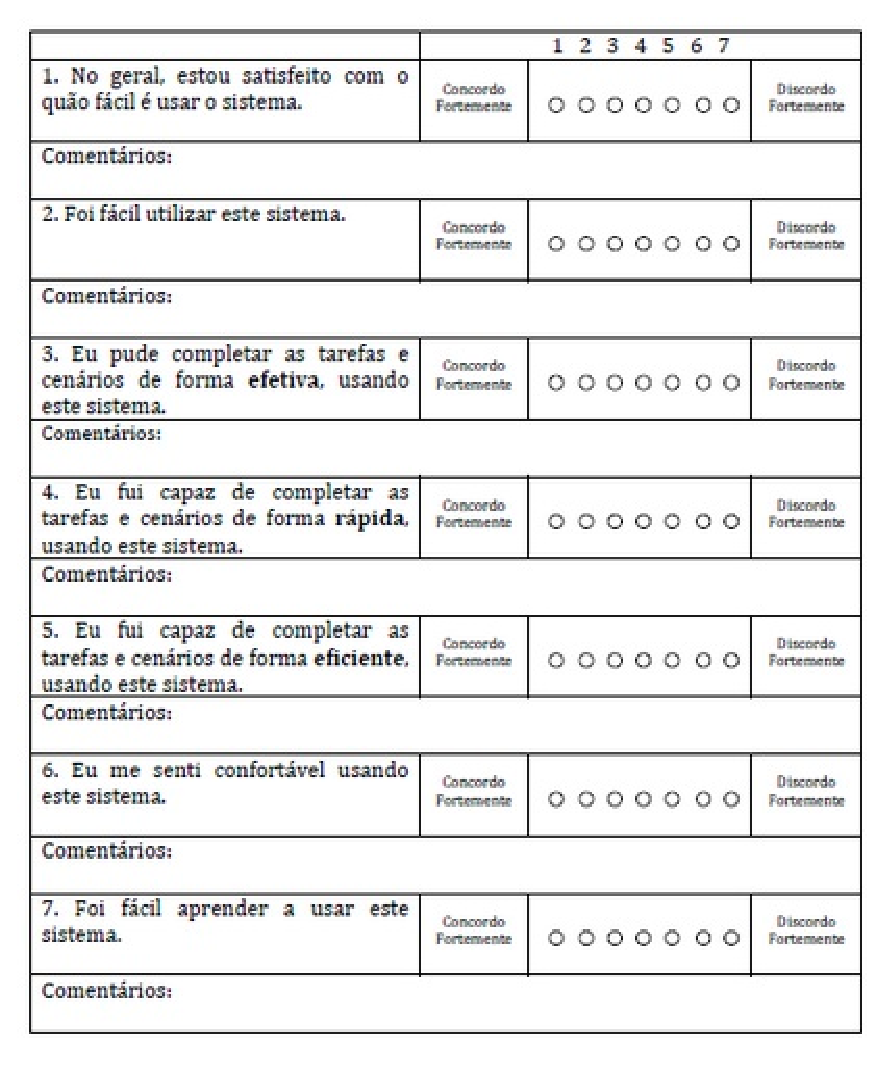
\includegraphics[keepaspectratio=true,scale=0.60]
      {figuras/pssuq01.eps}
    \label{pssuq}
	\caption{PSSUQ – The Post-Study System Questionnaire}
\end{figure}

\newpage

\begin{figure}[!h]
    \centering
    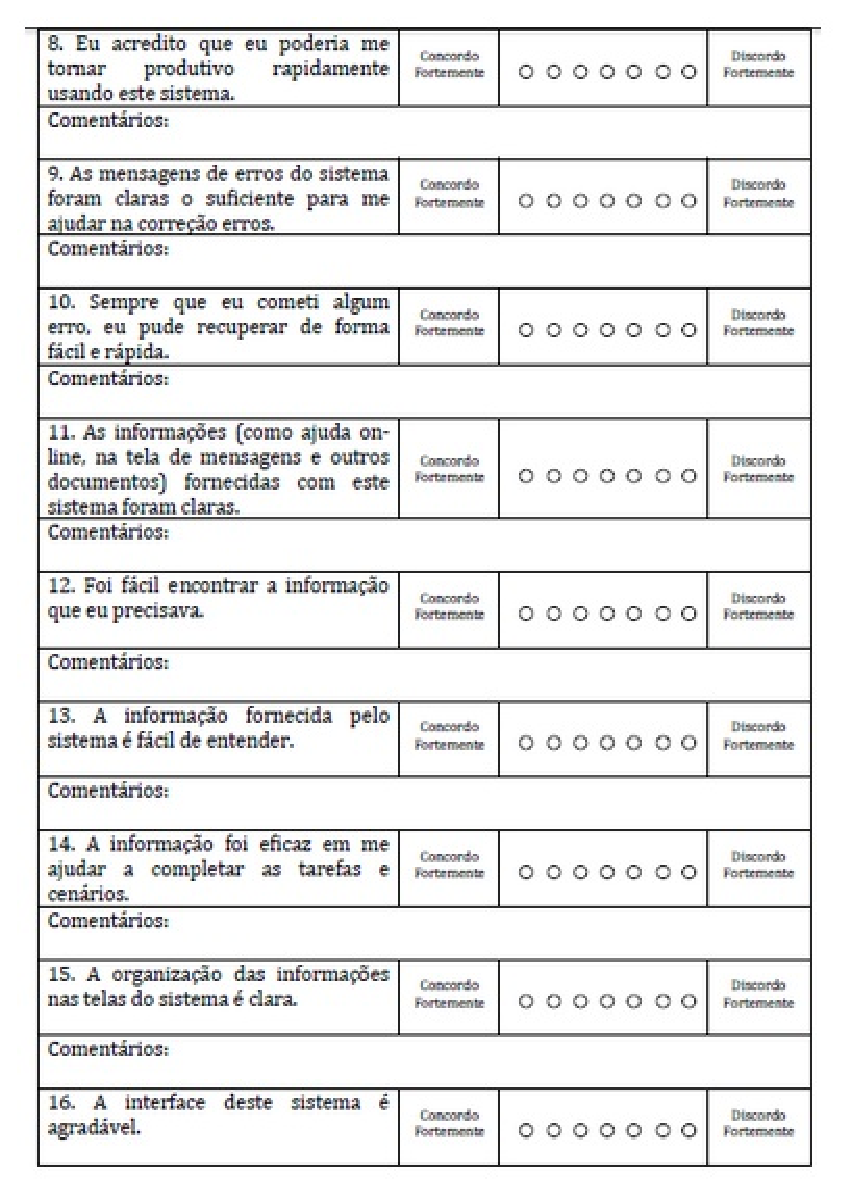
\includegraphics[keepaspectratio=true,scale=0.60]
      {figuras/pssuq02.eps}
    \label{pssuq}
\end{figure}

\begin{figure}[!h]
    \centering
    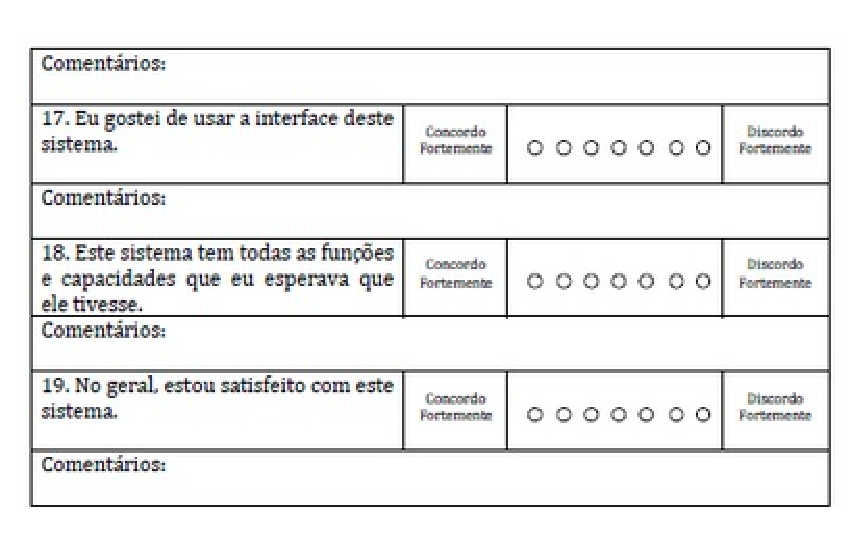
\includegraphics[keepaspectratio=true,scale=0.60]
      {figuras/pssuq03.eps}
    \label{pssuq}
	\caption{PSSUQ: The Post-Study System Questionnaire - Questões de 8 à 19}
\end{figure}

\subsection{CSUQ - Computer System Usability Questionnaire}

	Este questionário é parecido com o PSSUQ, mas a sua redação e diferente. Enquanto no PSSUQ afirma que “ Eu poderia efetivamente realizar as tarefas e cenários usando este sistema ” o CSUQ escreve: “ Eu posso terminar meu trabalho de forma eficaz usando esse sistema?”. Na IBM, este questionário foi aplicado através de e-mail, enviado para funcionários de diferentes locais, o que houve uma maior quantidade de participantes, do que feito com grupos reduzidos presencialmente. ~\cite{lewis1995ibm} 
	O CSUQ é utilizado quando o estudo de usabilidade é em um ambiente fora do laboratório. A confiabilidade relatada foi de 0,93.



\subsection{Comparativo dos questionários}

	Os questionários ASQ e PSQ são utilizados após a realização de um cenário. Contém os mesmos itens, mas possuem escalas diferentes. O ASQ possui uma maior confiabilidade em relação ao PSQ. 

	PSSUQ e CSUQ são ambos os questionários de satisfação global. O PSSUQ utiliza itens adequados para uma situação de teste de usabilidade, já o CSUQ são apropriados para uma situação de teste de campo. Os questionários possuem propriedades psicométricas aceitáveis de usabilidade e podem ser usados com confiança como medidas padronizadas de satisfação. É interessante utilizar o PSSUQ junto com o ASQ.

	O ideal é que o questionário seja mais genérico possível. Cada questionário possui um nível de confiança.

\begin{table}[h]
\begin{tabular}{l|l|l|l|p{3cm}|l|l|}
\hline
\textbf{Nome} & \textbf{Criador} & \textbf{Questões} & \textbf{Licença} & \begin{tabular}[c]{@{}l@{}}\textbf{Interface  Avaliada}\end{tabular}  & \textbf{Confiab.} & \textbf{Escala} \\ \hline
ASQ & IBM & 3 & Aberto & Qualquer & 0,93 & \begin{tabular}[c]{@{}l@{}}Discordo \\ Fortemente /\\ Concordo \\ Fortemente\end{tabular} \\ \hline
\begin{tabular}[c]{@{}l@{}}CSUQ\end{tabular}    & IBM              & 19       & Aberto          & \begin{tabular}[c]{@{}l@{}}Baseado em\\ computador \end{tabular} & 0,95           & \begin{tabular}[c]{@{}l@{}}Discordo \\Fortemente /\\ Concordo \\ Fortemente\end{tabular} \\ \hline
\begin{tabular}[c]{@{}l@{}}PSSUQ\end{tabular} & IBM              & 19       & Aberto          & \begin{tabular}[c]{@{}l@{}}Baseado em\\ computador \end{tabular} & 0,96           & \begin{tabular}[c]{@{}l@{}}Discordo \\ Fortemente /\\ Concordo\\ Fortemente\end{tabular} \\ \hline
\begin{tabular}[c]{@{}l@{}}SUMI\end{tabular}   & HERG             & 27       & Proprietário    & Software              & 0,89           & \begin{tabular}[c]{@{}l@{}}Discordo \\Fortemente /\\ Concordo\\ Fortemente\end{tabular} \\ \hline
SUS                                                                 & DEC              & 10       & Aberto          & Qualquer              & 0,85           & \begin{tabular}[c]{@{}l@{}}Discordo \\Fortemente / \\Concordo \\Fortemente    \end{tabular}                                         \\ \hline
QUIS                                                                                         & UMD              & 50       & Proprietário    &       -         &       -         & 0 a 9                                                                               \\ \hline
\end{tabular}
\caption {Comparativo dos questionários}
\end{table}

\begin{comment}

\section{Portal da Participação Social}


\subsection{Persona}

	A estrutura da persona foi feita seguindo o modelo criado por Edu Agni, autor do blog uxdesign.blog.br para o curso de UX Design na qual ele ministra em várias cidades do país.

\begin{itemize}

\item Persona 1

Nome: Leo Silva

Idade: 27 anos

Localidade: São Paulo

Citação: "Minha vida é andar por este país"

Interesses e motivações: Comunismo, culinária e política

Frustações: Problemas sociais do Brasil

Background: Estudou Serviço Social

Objetivos do usuário: Informas às pessoas sobre as lutas sociais propostas pelo seu grupo.

\item Persona 2

Nome: José Teixeira

Idade: 45 anos

Localidade: Bahia

Ocupação: Deputado

Interesses: Política, movimentos sociais

Background: Líder de movimentos sociais, sindicatos e associações

Objetivos do usuário: Debater leis, projetos e emendas participativas, criação de enquetes.

\end{itemize}


\subsection{Cenários}

	Os cenários foram levantados através de uma análise do que era permitido de realizar no portal e quais seriam mais importantes para as principais atividades de um usuário. Foram pensadas levando em consideração as necessidades dos usuários do portal da participação social. Tarefas que os usuários-alvo executariam mais frequentemente e tarefas que poderiam apresentar problemas para a compreensão e execução do usuário. 

	Através das redes sociais e do perfil do usuário no portal da participação social foi identificado que uma das atividades mais realizadas pelos usuários são de edição de textos no blog do perfil, além da criação de mecanismos de participação social como a votação em pares (parwise).
	
	Entender o perfil do usuário é um dos principais pontos que devem ser levados em consideração pelos desenvolvedores de software em geral. Cada perfil de usuário tem suas particularidades e suas expectativas quanto a utilização do sistema.

\begin{enumerate}
	\item Faça seu cadastro no portal Participa.Br e ative sua conta.
	\item Personalize o seu perfil inserindo uma foto, escolha 5 categorias de interesse.
	\item Localize e adicione Jônatas Medeiros de Mendonça à sua rede.
	\item Localize e ingresse na comunidade Participação Social. Informe a quantidade de membros.
	\item Localize a pessoa Henrique Parra Filho e infome a quantidade de amigos, nº de comunidades.
	\item José deseja criar um artigo para seu blog. Ele possui o texto já criado em doc, mas precisa inserir alguns outros detalhes em seu artigo como: links, imagens, tamanhos de fonte e subtítulos e inserir a licença de uso.
	\item João necessita criar um outro artigo e inserir a mesma imagem.
	\item Visualizar galeria de imagens, remova a imagem adicionada e adicione novas imagens.
	\item Entre no portal e acesse o painel de controle e modifique a aparência de seu perfil.
	\item Escreva uma descrição para o seu blog e inseria uma imagem.
	\item Crie um conteúdo para sua página e adicione um item de menu para esse novo conteúdo.
	\item Adicione um novo bloco na página de seu perfil.
	\item Crie um questionário \textit{Pairwise}.
\end{enumerate}


\subsection{Problemas levantados com as questões}

Ao realizar uma verificação das tarefas levantadas foram analisados alguns problemas de usabilidade que o portal apresentava: 

\begin{enumerate}

\item Ao editar um texto, apenas voltando no navegador e tentar salvar novamente não será mais possível devido o sistema considerar como um novo artigo e aparece uma mensagem de erro. O problema encontrado nessa mensagem de erro se dá pelo fato da mensagem vir em inglês, dificultando a leitura por muitas pessoas. 

\item Ao colocar o item como justificado não funcionava, então não é possível saber se o texto realmente ficaria justificado. 

\item No começo, uma das dúvidas era aonde inserir a imagem, a primeira tentativa foi pelo ícone de imagem do próprio editor de texto, que ao
abrir o pop up precisava ser redimensionado. Utilizando essa função do editor o usuário precisaria saber do link da imagem o que inviabilizaria. Essa opção então deve ser usada apenas para redimensionar a imagem.

\item Ao inserir uma imagem não é informado ao usuário quais as mídias podem ser inseridas e nem o tamanho permitido.

\item Na inserção de uma imagem, quando arrasta o nome da mídia para o texto, aparece um link escrito (adicionar Artigo) ao invés da imagem;

\item Na busca da imagem, caso o usuário não lembre o nome da imagem será impossível adiciona-la. Se o usuário escolher inserir mídia e escolher a mesma imagem acontecerá um erro e não será possível adicionar a imagem devido que ela já existe na pasta. Mas não é informado o por que não conseguiu inserir a imagem.

\item Na galeria de imagens existe um botão chamado remover que pode confundir o usuário pensando que serviria para remover a imagem, e ao clicar era removido toda a galeria. O navegador deu aviso, mas veio em inglês.

\item  Outro problema encontrado não se refere a questão de usabilidade em si, mas de aparência no tema \textit{Conference} na qual os ícones dos menus não estão formatados.

\item Na criação do questionário pairwise, o problema encontrado é que não há explicação do que seria esse tipo de questionário.

\end{enumerate}

\subsection {Ferramenta de análise de websites}

Utilizamos uma ferramenta de análise de websites, Woorank\footnote{\url{http://www.woorank.com/}}, para verificar alguns problemas existentes no portal da participação social.

\begin{figure}[!h]
    \centering
    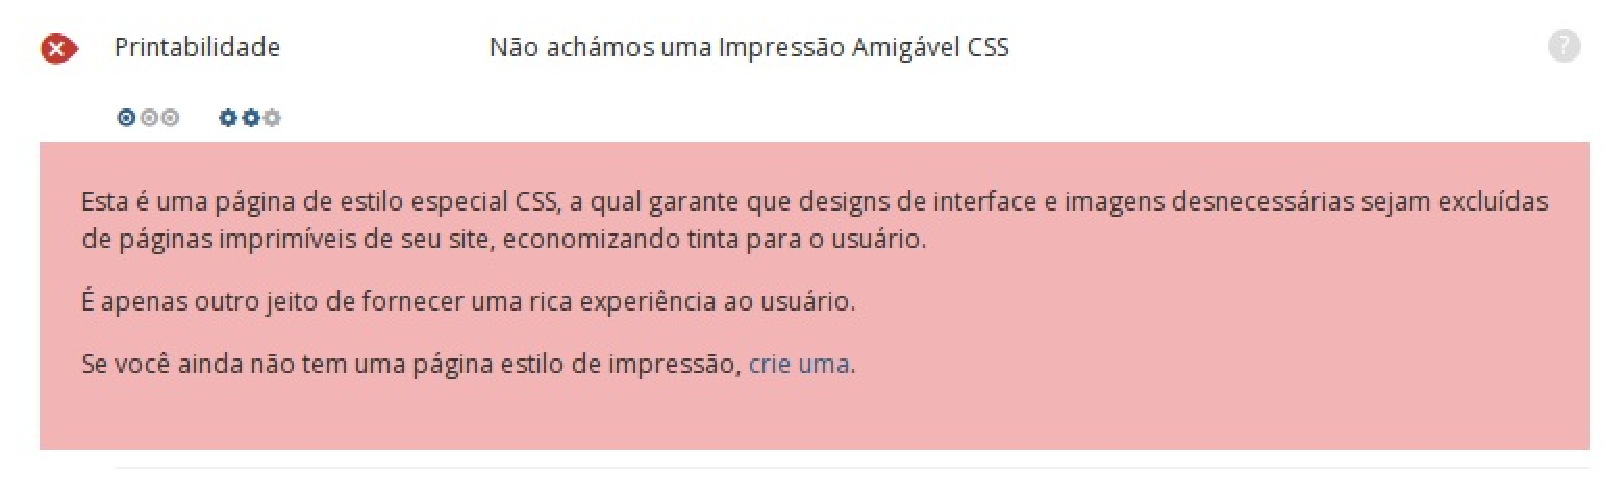
\includegraphics[keepaspectratio=true,scale=0.60]
      {figuras/printabilidade.eps}
    \caption{Printabilidade - Portal da Participação Social}
    \label{printabilidade}
\end{figure}

\begin{figure}[!h]
    \centering
    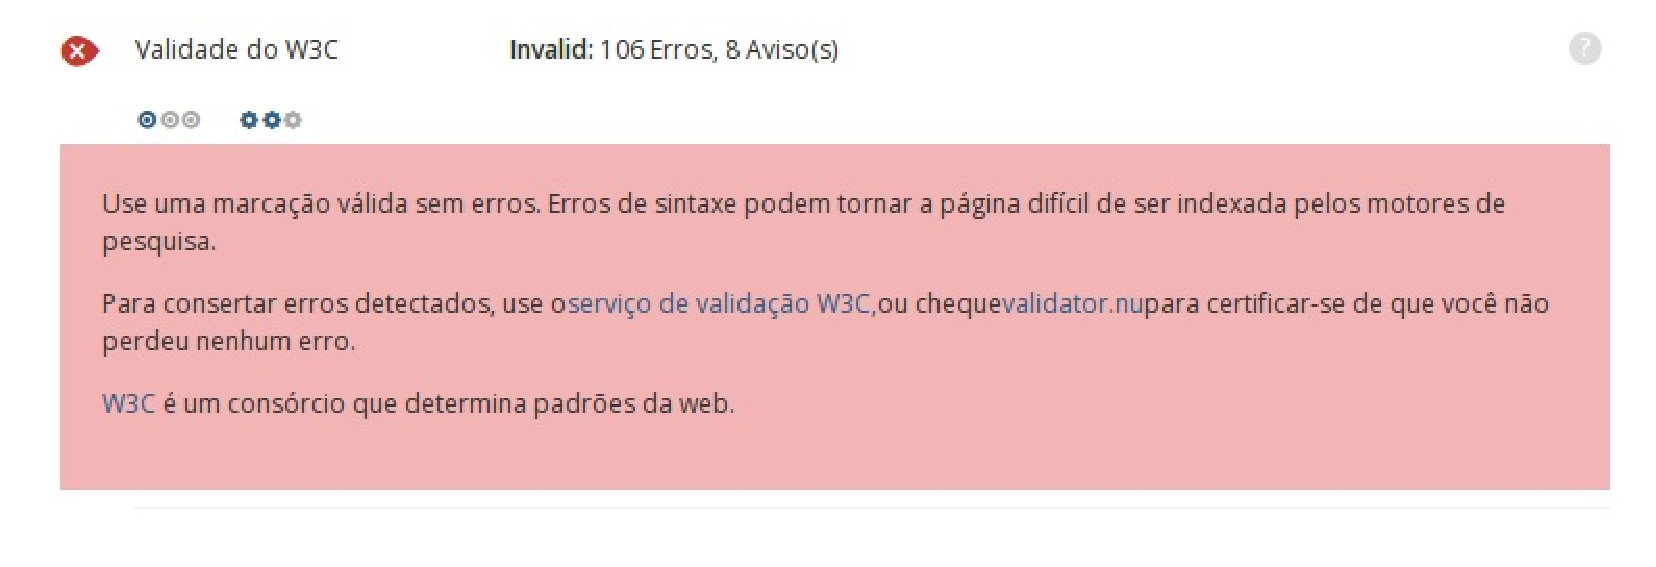
\includegraphics[keepaspectratio=true,scale=0.60]
      {figuras/validacoes.eps}
    \caption{Validações - Portal da Participação Social}
    \label{validacoes}
\end{figure}

\begin{figure}[!h]
    \centering
    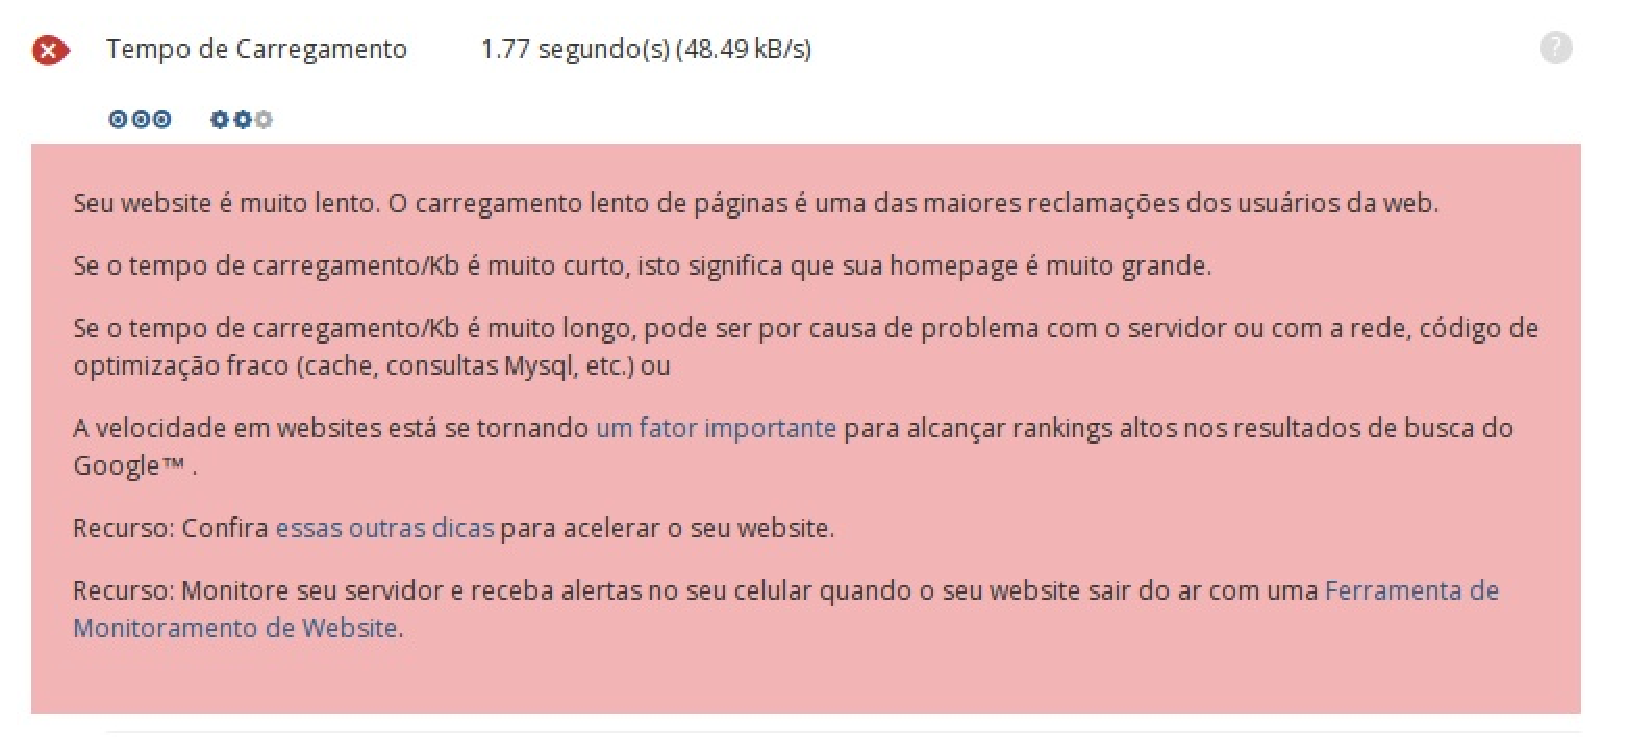
\includegraphics[keepaspectratio=true,scale=0.60]
      {figuras/carregamento.eps}
    \caption{Carregamento de Página - Portal da Participação Social}
    \label{carregamento}
\end{figure}

Em relação ao acesso em dispositivos móveis foram encontrados alguns problemas como lentidão e não renderização na página em celulares.

\begin{figure}[!h]
    \centering
    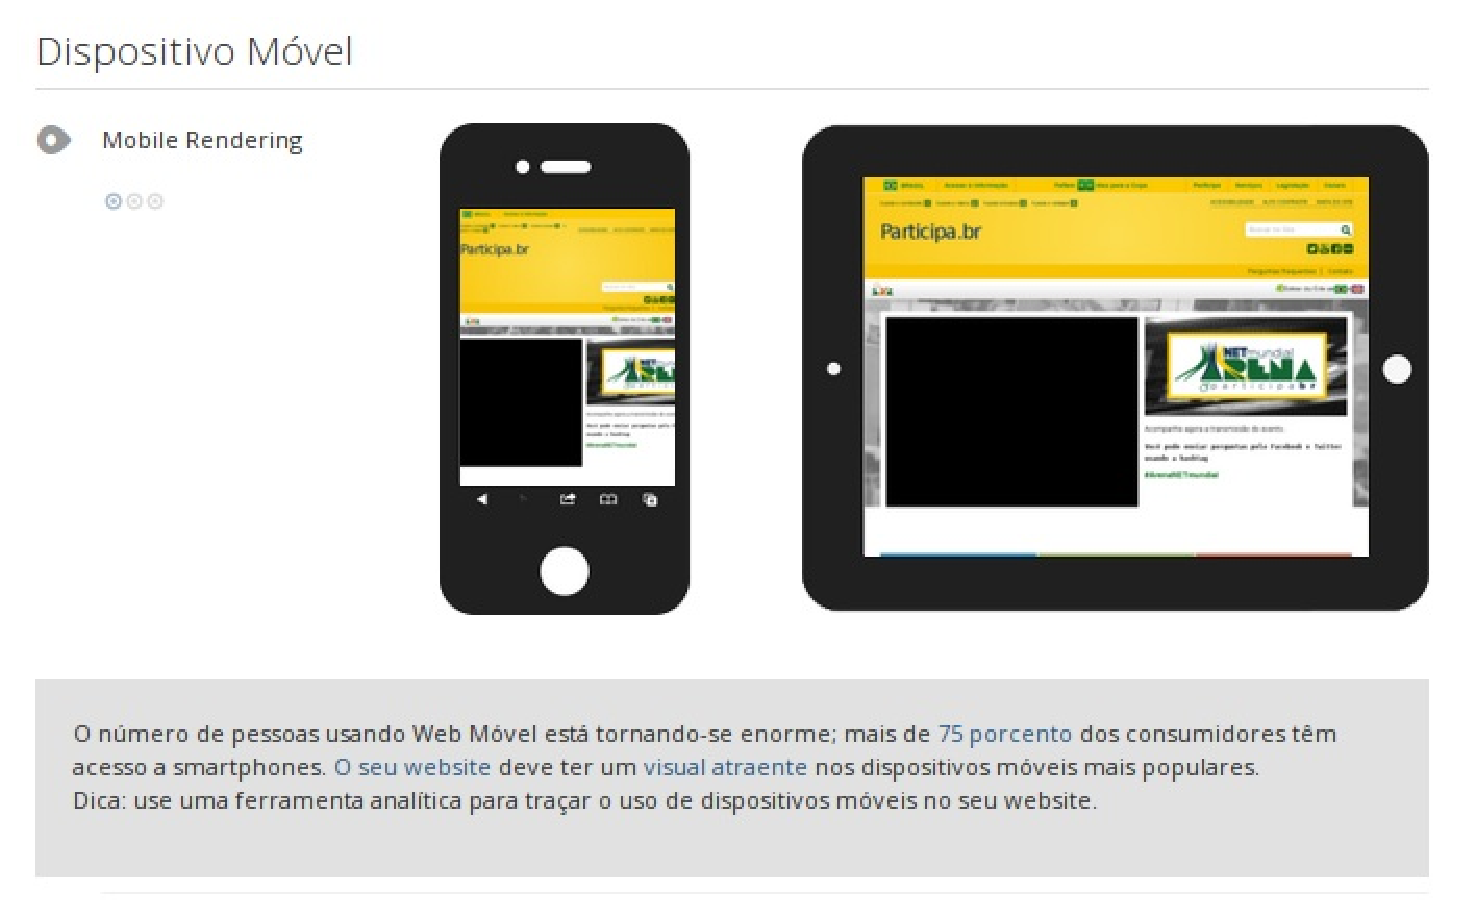
\includegraphics[keepaspectratio=true,scale=0.60]
      {figuras/movel.eps}
    \caption{Renderização de página em dispositivos móveis}
    \label{movel}
\end{figure}

\begin{figure}[!h]
    \centering
    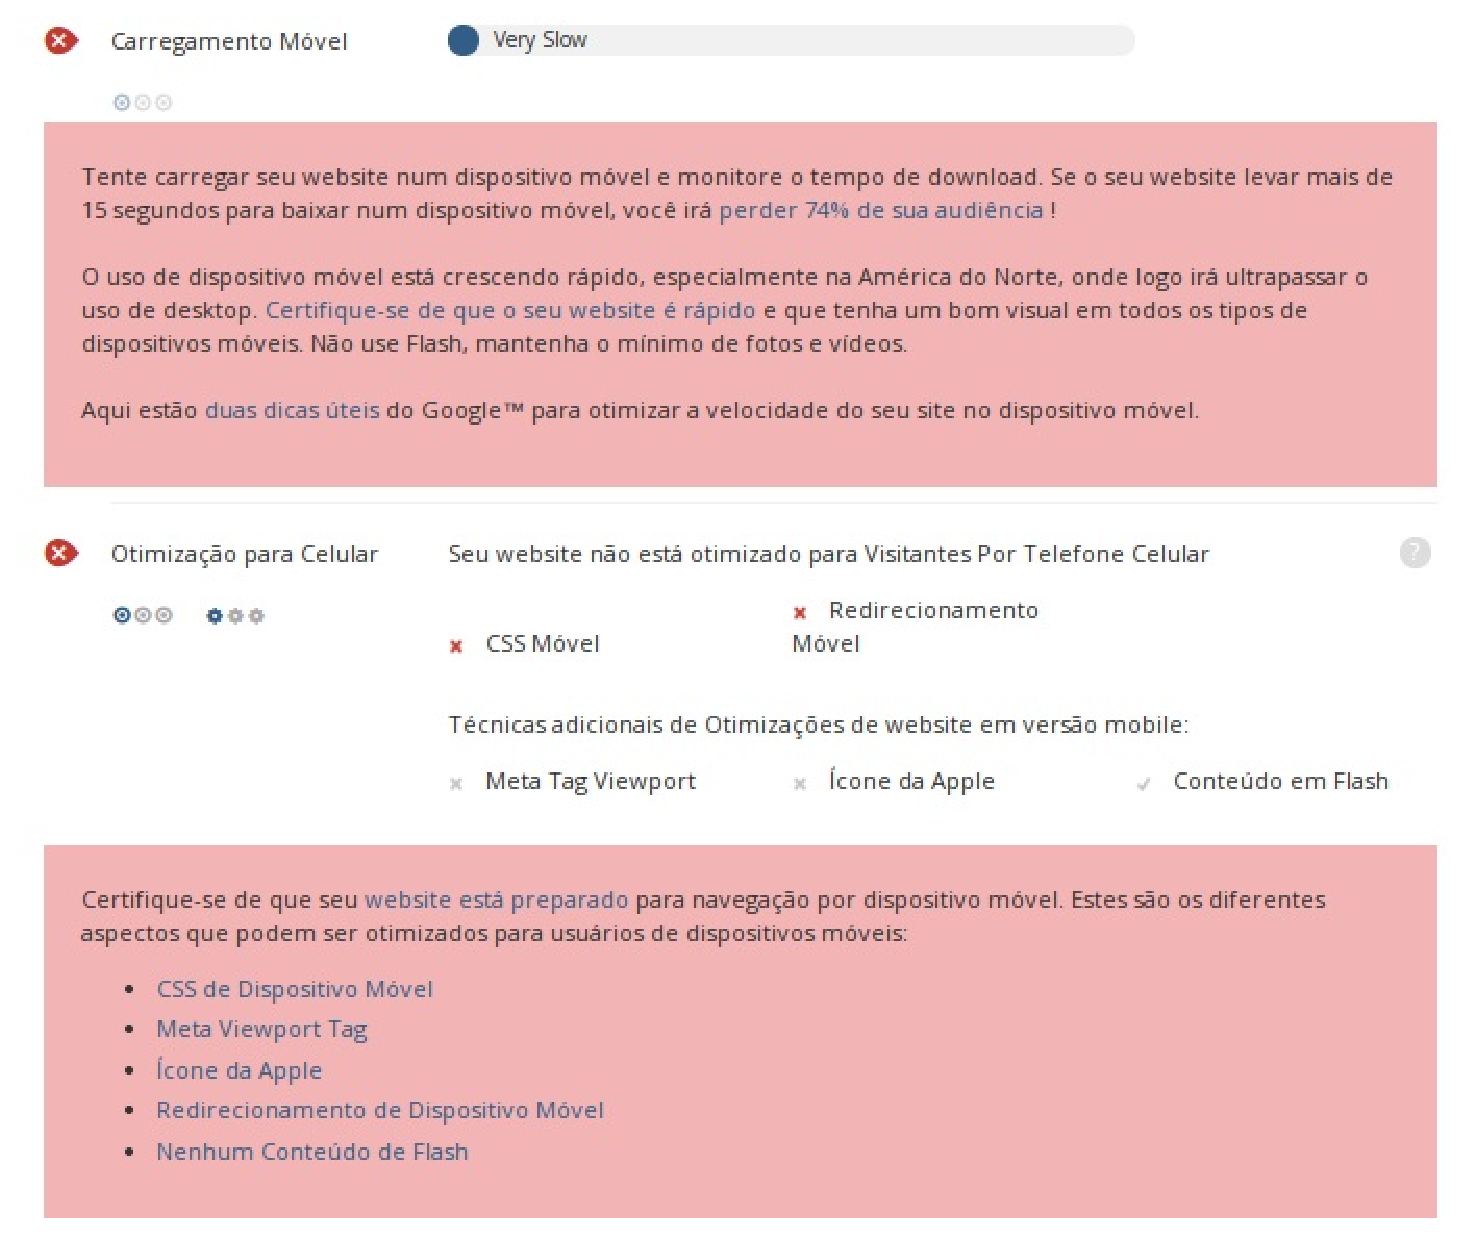
\includegraphics[keepaspectratio=true,scale=0.60]
      {figuras/carregamentomovel.eps}
    \caption{Carregamento por dispositivos móveis - participa.br}
    \label{carregamentomovel}
\end{figure}

\end{comment}
